\documentclass[uplatex,dvipdfmx]{jsarticle}

\usepackage[uplatex,deluxe]{otf} % UTF
\usepackage[noalphabet]{pxchfon} % must be after otf package
\usepackage{stix2} %欧文&数式フォント
\usepackage[fleqn,tbtags]{mathtools} % 数式関連 (w/ amsmath)
\usepackage{hira-stix} % ヒラギノフォント&STIX2 フォント代替定義(Warning回避)
\usepackage{graphics}

\begin{document}

\title{レポート2}
\date{2025年1月13日}
\maketitle
\section{はじめに}
BBS(電子掲示板)に3つの機能を追加した.
本書では,このBBSについて仕様書を記述する.
また,その内容は利用者向け,管理者向け,開発者向けの3章構成で説明している.
\section{機能概要}
既存の掲示板に関して以下の機能を追加した.\par

\begin{itemize}
	\item 書き込み日時表示機能
	\begin{itemize}
		\item 投稿チェックでの名前の左側に,書き込んだ時の日時を表示する機能である
		\item いつ発言したかがわからなかったがそれが分かるようにこの機能を追加した
	\end{itemize}
	\item 職業選択機能
	\begin{itemize}
		\item 職業を選択するリストを追加し,名前の右側に表示できる機能である
		\item 発言者の立場を表記することでコミュニケーションを円滑にするためにこの機能を追加した
	\end{itemize}
	\item 表示数変更機能
	\begin{itemize}
		\item 1つの画面に表示する投稿数を制限する機能である
		\item  発言数が多くなることでページが多くなることを防ぐためにこの機能を追加した
	\end{itemize}
\end{itemize}


\section{利用者向け編}
\subsection{操作説明}
本BBSの操作説明を記述する.\par

\begin{enumerate}
	\item 以下のURLにアクセスする
	\begin{itemize}
		\item http://localhost:8080/public/bbs.html 
	\end{itemize}
	\item 図1のような初期画面になる
	\item 名前とメッセージを入力し,職業と表示数を選択する
	\item 送信ボタンをクリックし,投稿チェックボタンをクリックする
	\item 3,4を繰り返すことで図2の例のように表示される
\end{enumerate}


\begin{figure}[h]
\centering
 \centering
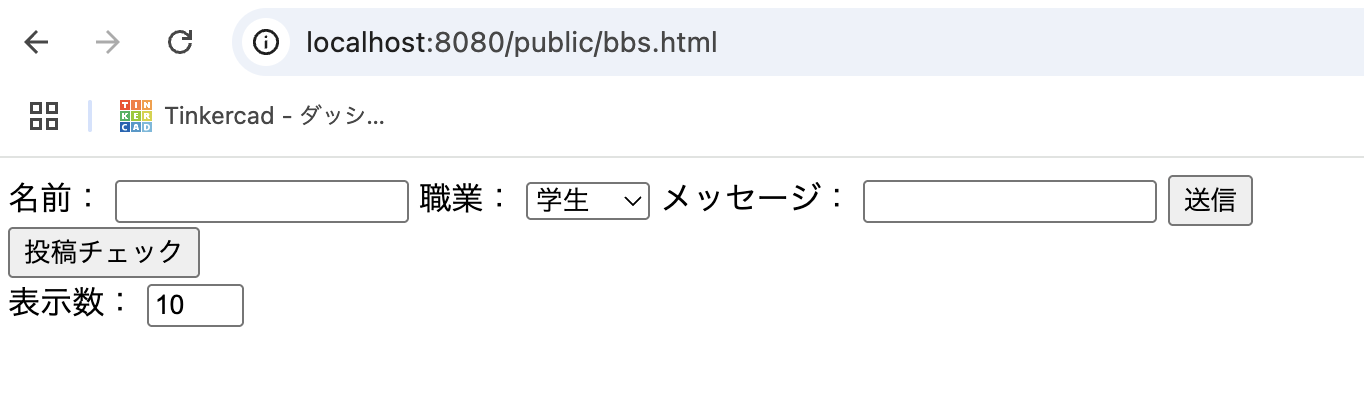
\includegraphics[width=10cm]{./syoki.png}
\caption{BBSの初期画面}
\label{fig:problem}
\end{figure}


\begin{figure}[h]
\centering
 \centering
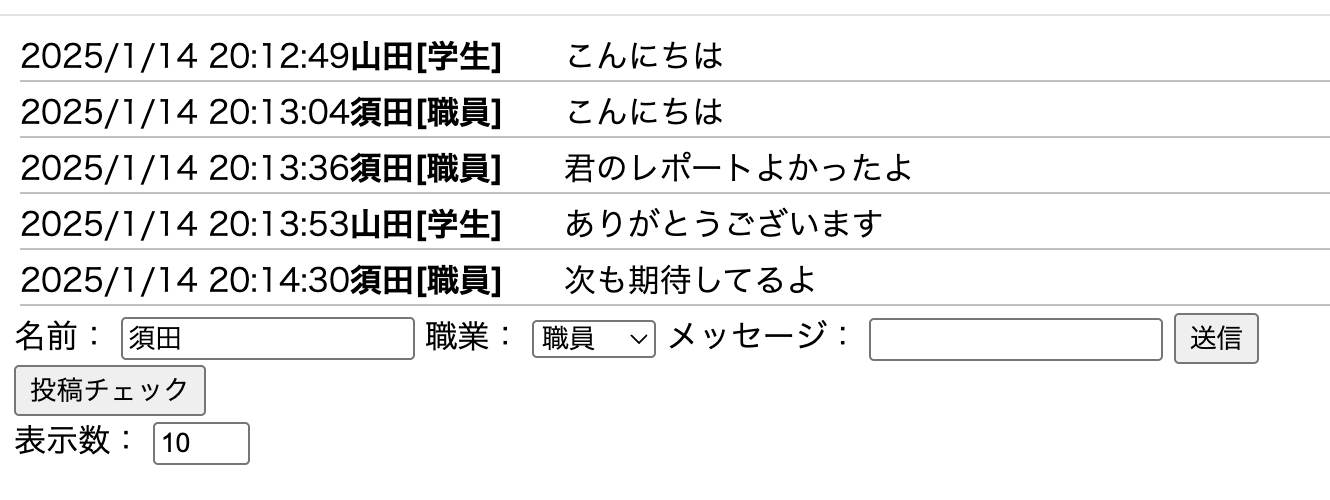
\includegraphics[width=10cm]{./rei.png}
\caption{BBSの使用例}
\label{fig:problem}
\end{figure}



\section{管理者向け編}
\subsection{インストール方法}

\begin{enumerate}
	\item ターミナルに以下のコードを打ち込み,ソースコードのクローンを取得する
	\begin{itemize}
		\item git clone https://github.com/teru0701/webpro\_06.git
	\end{itemize}
	\item 以下のコードを打ち込み,クローンが置かれたgitのフォルダに移動する
	\begin{itemize}
		\item cd webpro\_06
	\end{itemize}
	\item 以下のコードを打ち込み,パッケージをインストールする
	\begin{itemize}
		\item  npm install
	\end{itemize}
\end{enumerate}

\subsection{起動方法}

\begin{enumerate}
	\item cdコマンドでインストールしたフォルダーまで移動する
	\item 以下のコードを打ち込み,サーバを起動する
	\begin{itemize}
		\item  node app8.js
	\end{itemize}
	\item 終了時はCommand+Cを打ち込み,サーバを終了させる
\end{enumerate}

\newpage

\section{開発者向け編}
\subsection{プログラム構成}

\begin{table}[h]
\centering
\begin{tabular}{|l|l|}
\hline
\textbf{ファイル名}       & \textbf{説明}                           \\ \hline
\texttt{app8.js}          & クライアント側の情報を受け取り,掲示板として管理するサーバプログラム                        \\ \hline
\texttt{public/bbs.html} & 開始画面               \\ \hline
\texttt{public/bbs.css} & 開始画面のデザイン       \\ \hline
\texttt{public/bbs.js} & クライアント側で実行するプログラム               \\ \hline
\end{tabular}
\caption{ファイル名とその説明}
\label{tab:file-description}
\end{table}


\subsection{プログラム詳細}
\subsubsection{サーバAPI(check処理)}

\begin{enumerate}
	\item 処理概要:投稿チェックをクリックすると全投稿数が取得できる
	\item 入力:なし
	\item 出力:全投稿数
	\item 備考:今回の機能追加で修正点は特になし
\end{enumerate}

\subsubsection{サーバAPI(post処理)}

\begin{enumerate}
	\item 処理概要:入力した発言内容をサーバ側に渡し,管理する(保存した発言内容はread処理で取得できる)
	\item 入力:投稿者,投稿内容,日付,職業
	\item 出力:全投稿数
	\item 備考:日付と職業をサーバーに渡すようクライアントを修正し,それに伴いサーバ側も合わせて修正した
\end{enumerate}

\subsubsection{サーバAPI(read処理)}

\begin{enumerate}
	\item 処理概要:指定した開始番号以降の発言を取得する
	\item 入力:開始番号(0)
	\item 出力:投稿者と投稿内容と日付と職業の塊が複数
	\item 備考:以前は新しい発言だけをサーバーから取得するために開始番号を指定していたが,今回はクライアント側で表示する数を指定するため,開始番号は「0」で固定し,すべての発言を取得するように修正した.なお、本方式ではサーバからすべての発言を取得するため,必要以上に通信量が多くなってしまう.そのため,開始番号を適切な番号(発言件数ー表示数)を指定することでサーバから表示に必要な発言だけを取得するように修正する予定である.
\end{enumerate}


\end{document} 
